\documentclass[11pt]{article}
\usepackage{../cs70, latexsym,epsf,amsmath,amsfonts,graphicx,url,textcomp}
\lecture{19}
\def\title{Note \the\lecturenumber}

%%% Alistair's Macros
\makeatletter
\def\eqalign#1{\,\vcenter{\openup\jot\m@th
  \ialign{\strut\hfil${##}$&${{}##}$\hfil
      \crcr#1\crcr}}\,}
\def\eqalignno#1{\displ@y \tabskip\@centering
  \halign to\displaywidth{\hfil${##}$\tabskip\z@skip
    &${{}##}$\hfil\tabskip\@centering
    &\llap{$##$}\tabskip\z@skip\crcr
    #1\crcr}}
\makeatother
\def\third{{\textstyle{1\over 3}}}
\def\half{{\textstyle{1\over 2}}}
\def\quarter{{\textstyle{1\over 4}}}
\def\ul#1{\underline{#1}}
\def\VarOmega{\mathchar"10A }
\def\varOmega{\mathchar"10A }
\newenvironment{proposition}{\par\global\advance\theoremnumber by 1
{\bf Proposition \the\lecturenumber.\the\theoremnumber}:
\begingroup\em}%
{\endgroup}
\def\ignore#1{}
\def\Ex#1{{\rm E}(#1)}
\def\Var#1{{\rm Var}(#1)}
\def\Aset{{\cal A}}
%%% End Alistair's Macros


\newcounter{thm}
\addtocounter{thm}{\the\lecturenumber}
\newtheorem{corollary}{Corollary}[thm]
\newtheorem{theorem}{Theorem}[thm]
\newtheorem{definition}{Definition}[thm]



\begin{document}
\maketitle

\section*{Some Important Distributions}

Recall our basic probabilistic experiment of tossing a biased coin $n$ times. This is a very simple
model, yet surprisingly powerful. Many important probability distributions that are
widely used to model real-world phenomena can be derived from looking at this basic coin
tossing model.

The first example, which we have seen in Note~16, is the {\em binomial distribution} $Bin(n,p)$.
This is the distribution of the number of Heads, $S_n$, in $n$ tosses of a biased coin with probability $p$ to be Heads. 
Recall that the distribution of $S_n$ is $\Pr[S_n = k] = {n \choose k} p^k (1-p)^{n-k}$ for $k \in \{0,1,\dots,n\}$. The expected value is $\Ex{S_n} = np$ and the variance is $\Var{S_n} = np(1-p)$. The binomial distribution frequently appears
to model the number of successes in a repeated experiment.


\subsection*{Geometric Distribution}

Consider tossing a biased coin with Heads probability~$p$ repeatedly. Let $X$ denote
the number of tosses until the first Head appears. Then $X$ is a random variable that 
takes values in the set of positive integers $\{1,2,3,\dots\}$. The event that
$X = i$ is equal to the event of observing Tails for the first $i-1$ tosses and getting Heads
in the $i$-th toss, which occurs with probability $(1-p)^{i-1}p$. Such a random variable is
called a geometric random variable.

The geometric distribution frequently occurs in applications because
we are often interested in how long we have to wait before a
certain event happens: how many runs before the system fails, how many
shots before one is on target, how many poll samples before we find
a Democrat, how many retransmissions of a packet before successfully
reaching the destination, etc.



\begin{definition}[Geometric distribution] A random variable $X$ for which $$
   \Pr[X=i] = (1-p)^{i-1}p\qquad\hbox{\rm for $i=1,2,3,\ldots$}  $$
is said to have the \ul{geometric distribution with parameter~$p$}. This is abbreviated as $X \sim Geom(p)$.
\end{definition}

As a sanity check, we can verify that the total probability of $X$ is equal to $1$:
$$\sum_{i=1}^\infty \Pr[X = i] = \sum_{i=1}^\infty (1-p)^{i-1} p = p \sum_{i=1}^\infty (1-p)^{i-1} = p \times \frac{1}{1-(1-p)} = 1,$$
where in the second-to-last step we have used the formula for geometric series.

If we plot the distribution of~$X$ (i.e., the values $\Pr[X=i]$
against~$i$) we get a curve that decreases monotonically by a
factor of $1-p$ at each step, as shown in Figure \ref{fig:geometric}.

\begin{figure}[h!]
\centering
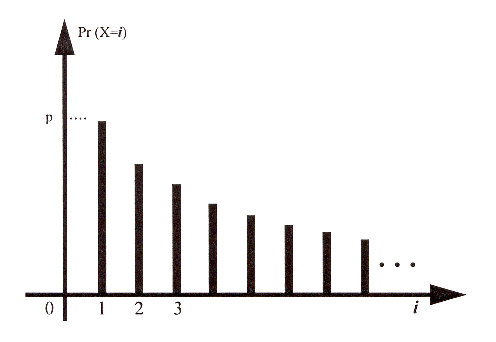
\includegraphics[scale=0.8]{geometric}
\caption{The Geometric distribution.}
\label{fig:geometric}
\end{figure}

Let us now compute the expectation $\Ex{X}$. Applying the definition of expected value
directly gives us:
$$ \Ex{X} = \sum_{i=1}^\infty i \times \Pr[X = i] = p\sum_{i=1}^\infty i(1-p)^{i-1}.$$
However, the final summation is difficult to evaluate and requires some calculus trick.
Instead, we will use the following alternative formula for expectation.



\begin{theorem}\label{thm:exp}
Let $X$ be a random variable that takes values in $\{0,1,2,\dots\}$. Then $$
   \Ex{X} = \sum_{i=1}^\infty \Pr[X\ge i].  $$
\end{theorem}
\begin{proof}
For notational convenience, let's write $p_i=\Pr[X=i]$, for $i=0,1,2,\ldots$.
From the definition of expectation, we have $$
\eqalign{\Ex{X}&=(0\times p_0) + (1\times p_1) + (2\times p_2) + (3\times p_3) + (4\times p_4) + \cdots\cr
               &= p_1 +(p_2+p_2) + (p_3+p_3+p_3) + (p_4+p_4+p_4+p_4)+\cdots\cr
               &= (p_1+p_2+p_3+p_4+\cdots) + (p_2+p_3+p_4+\cdots) + (p_3+p_4+\cdots) + (p_4+\cdots) +\cdots\cr
               &= \Pr[X\ge 1] + \Pr[X\ge 2] + \Pr[X\ge 3] + \Pr[X\ge 4] +\cdots.\cr}  $$
In the third line, we have regrouped the terms into convenient infinite
sums, and each infinite sum is exactly the probability that $X \ge i$ for each $i$. You should check that you understand how the fourth line follows from the third.  

Let us repeat the proof more formally, this time using more compact mathematical notation:
\begin{equation*}
\Ex{X} = \sum_{j=1}^\infty j \times \Pr[X=j] = \sum_{j=1}^\infty \sum_{i = 1}^j \Pr[X=j] = \sum_{i=1}^\infty \sum_{j = i}^\infty \Pr[X=j] = \sum_{i=1}^\infty \Pr[X\ge i].
\vspace{-15pt}
\end{equation*}
\end{proof}

We can now use Theorem~\ref{thm:exp} to compute $\Ex{X}$ more easily.
\begin{theorem}
For a geometric random variable~$X \sim Geom(p)$, we have $\Ex{X} = \frac{1}{p}$.
\end{theorem}
\begin{proof}
The key observation is that for a geometric random variable $X$,
\begin{equation}\label{eq1}
   \Pr[X\ge i] = (1-p)^{i-1} ~ \text{ for } i = 1,2,\dots.
\end{equation}
We can obtain this simply by summing $\Pr[X = j]$ for $j \ge i$. Another way
of seeing this is to note that the event ``$X\ge i$'' means at least $i$
tosses are required.  This is equivalent to saying that the
first $i-1$ tosses are all Tails, and the probability of this event
is precisely $(1-p)^{i-1}$.  Now, plugging equation~(\ref{eq1}) into
Theorem~\ref{thm:exp}, we get $$
   \Ex{X} = \sum_{i=1}^\infty\Pr[X\ge i] = \sum_{i=1}^\infty (1-p)^{i-1}
                                         = {1\over{1-(1-p)}} ={1\over p},  $$
where we have used the formula for geometric series.                                         
\end{proof}

So, \ul{the expected number of tosses of a biased coin until the first
Head appears is~$1\over p$}. Intuitively, if in each coin toss we expect
to get $p$ Heads, then we need to toss the coin $\frac{1}{p}$ times to get
$1$ Head. So for a fair coin, the expected number of tosses is~2, but remember
that the actual number of coin tosses that we need can be any positive integers.

{\bf Remark:} Another way of deriving $\Ex{X} = \frac{1}{p}$ is to use the interpretation
of a geometric random variable $X$ as the number of coin tosses until we get a Head. Consider
what happens in the first coin toss: If the first toss comes up Heads, then $X = 1$. Otherwise,
we have used one toss, and we repeat the coin tossing process again; the number
of coin tosses after the first toss is again a geometric random variable with parameter
$p$. Therefore, we can calculate:
$$\Ex{X} = \underbrace{p \cdot 1}_{\text{first toss is H}} + \underbrace{(1-p) \cdot (1 + \Ex{X})}_{\text{first toss is T, then toss again}}.$$
Solving for $\Ex{X}$ yields $\Ex{X} = \frac{1}{p}$, as claimed.

Let us now compute the variance of $X$.

\begin{theorem}
For a geometric random variable~$X \sim Geom(p)$, we have $\Var{X} = \frac{1-p}{p^2}$.
\end{theorem}
\begin{proof}
We will show that $\Ex{X(X-1)} = \frac{2(1-p)}{p^2}$. Since we already know $\Ex{X} = \frac{1}{p}$, this will imply the desired result:
\begin{align*}
\Var{X} ~= \Ex{X^2} - \Ex{X}^2  
            ~&=~ \Ex{X(X-1)} + \Ex{X} - \Ex{X}^2 \\
            &= \frac{2(1-p)}{p^2} + \frac{1}{p} - \frac{1}{p^2}
            ~=~ \frac{2(1-p) + p - 1}{p^2}
            ~=~ \frac{1-p}{p^2}.
\end{align*}

Now to show $\Ex{X(X-1)} = \frac{2(1-p)}{p^2}$, we begin with the following identity of geometric series:
$$\sum_{i=0}^\infty (1-p)^i = \frac{1}{p}.$$
Differentiating the identity above with respect to $p$ yields (the $i = 0$ term is equal to $0$ so we omit it):
$$-\sum_{i=1}^\infty i (1-p)^{i-1} = -\frac{1}{p^2}.$$
Differentiating both sides with respect to $p$ again gives us (the $i = 1$ term is equal to $0$ so we omit it):
\begin{equation}\label{Eq:GeomHelp}
\sum_{i=2}^\infty i(i-1) (1-p)^{i-2} = \frac{2}{p^3}.
\end{equation}
Now using the geometric distribution of $X$ and identity~\eqref{Eq:GeomHelp}, we can calculate:
\begin{align*}
\Ex{X(X-1)} ~&=~ \sum_{i=1}^\infty i(i-1) \times \Pr[X = i]  \\
   ~&=~ \sum_{i=2}^\infty i(i-1) (1-p)^{i-1} p ~~~~~~~~~~~~~~~ \text{(the $i = 1$ term is equal to $0$ so we omit it)} \\
   ~&=~ p(1-p) \sum_{i=2}^\infty i(i-1) (1-p)^{i-2} \\
   ~&=~ p(1-p) \times \frac{2}{p^3} ~~~~~~~~~~~~~~~~~~~~~~~~~~~ \text{(using identity~\eqref{Eq:GeomHelp})} \\
   ~&=~ \frac{2(1-p)}{p^2},
\end{align*}
as desired.
\end{proof}



\subsubsection*{Application: The Coupon Collector's Problem}

Suppose we are trying to collect a set of $n$ different baseball cards.  We get the cards by
buying boxes of cereal: each box contains exactly one card, and it is
equally likely to be any of the $n$ cards.  How many boxes do we need
to buy until we have collected at least one copy of every card?

Let $X$ denote the number of boxes we need to buy in order to collect all $n$ cards.
The distribution of $X$ is difficult to compute directly (try it for $n = 3$). But if we are only interested in
its expected value $\Ex{X}$, then we can evaluate it easily using linearity of expectation
and what we have just learned about the geometric distribution.

As usual, we start by writing
\begin{equation}\label{eq2}
   X=X_1+X_2+\ldots+X_n
\end{equation}
for suitable simple random variables~$X_i$.  What should the $X_i$ be?
Naturally, $X_i$ is the number of boxes we buy while trying to get the $i$-th new card
(starting immediately after we've got the $(i-1)$-st new card). With this definition, make sure you
believe equation~(\ref{eq2}) before proceeding.

What does the distribution of~$X_i$ look like?  Well, $X_1$ is trivial:
no matter what happens, we always get a new card in the first box (since
we have none to start with).  So $\Pr[X_1=1]=1$, and thus $\Ex{X_1}=1$.

How about $X_2$?  Each time we buy a box, we'll get the same old card
with probability~$1\over n$, and a new card with probability~${{n-1}\over n}$.
So we can think of buying boxes as flipping a biased coin with Heads
probability $p={{n-1}\over n}$; then $X_2$ is just the number of
tosses until the first Head appears.  So $X_2$ has the geometric
distribution with parameter $p={{n-1}\over n}$, and $$
   \Ex{X_2}={n\over{n-1}}.  $$

How about $X_3$?  This is very similar to~$X_2$ except that now we only
get a new card with probability~${{n-2}\over n}$ (since there are
now two old ones).  So $X_3$ has the geometric distribution with
parameter $p={{n-2}\over n}$, and $$
   \Ex{X_3} = {n\over{n-2}}.  $$
Arguing in the same way, we see that, for $i=1,2,\ldots,n$, $X_i$ has the
geometric distribution with parameter $p={{n-i+1}\over n}$, and hence that $$
   \Ex{X_i} = {n\over{n-i+1}}.  $$
Finally, applying linearity of expectation to equation~(\ref{eq2}), we get
\begin{equation}\label{eq3}
   \Ex{X}=\sum_{i=1}^n\Ex{X_i}={n\over n} + {n\over{n-1}} +\cdots+{n\over 2}+{n\over 1} = n\sum_{i=1}^n{1\over i}.
\end{equation}
This is an exact expression for~$\Ex{X}$.  We can obtain a tidier form
by noting that the sum in it actually has a very good
approximation,\footnote{This is another of the little tricks you might
like to carry around in your toolbox.} namely:$$
   \sum_{i=1}^n{1\over i}\approx\ln n+\gamma, $$
where $\gamma=0.5772\ldots$ is known as {\it Euler's constant}.

Thus, \ul{the expected number of cereal boxes needed to
collect $n$ cards is about $n(\ln n+\gamma)$}.  This is an excellent
approximation to the exact formula~(\ref{eq3}) even for quite small
values of~$n$.  So for example, for $n=100$, we expect to buy about 518 boxes.


\subsection*{Poisson Distribution}

Consider the number of clicks of a Geiger counter, which measures radioactive emissions. 
The average number of such clicks per unit time, $\lambda$, is a measure of radioactivity, but the actual
number of clicks fluctuates according to a certain distribution called the Poisson distribution. 
What is remarkable is that the average value, $\lambda$, completely determines the probability distribution on
the number of clicks $X$. 

\begin{definition}[Poisson distribution] A random variable~$X$ for which
\begin{equation}\label{eq5}
   \Pr[X=i] = {{\lambda^i}\over{i!}}{\rm e}^{-\lambda}\qquad\hbox{\rm for
                            $i=0,1,2,\ldots$}
\end{equation}
is said to have the \ul{Poisson distribution with parameter~$\lambda$}. This is abbreviated as $X \sim Poiss(\lambda)$.
\end{definition}

To make sure this is a valid definition, let us check that (\ref{eq5})
is in fact a distribution, i.e., that the probabilities sum to~1.  We have $$
   \sum_{i=0}^\infty {{\lambda^i}\over{i!}}{\rm e}^{-\lambda} =
   {\rm e}^{-\lambda}\sum_{i=0}^\infty {{\lambda^i}\over{i!}} =
   {\rm e}^{-\lambda}\times{\rm e}^{\lambda} = 1.  $$
In the second-to-last step, we used the Taylor series expansion
${\rm e}^x = 1+x+{{x^2}\over{2!}}+{{x^3}\over{3!}}+\cdots$.

The Poisson distribution is also a very widely accepted model for so-called ``rare events," such as misconnected
phone calls, radioactive emissions, crossovers in chromosomes, the number of cases of disease, the number of births per 
hour, etc. This model is appropriate whenever the occurrences can be assumed to happen randomly with some 
constant density in a continuous region (of time or space), such that occurrences in disjoint subregions are independent. 
One can then show
that the number of occurrences in a region of unit size should obey the Poisson distribution with parameter $\lambda$.

\smallskip

{\bf Example:} Suppose when we write an article, we make an average of $1$ typo per page. We can model this with a Poisson random variable $X$ with $\lambda = 1$. So the probability that a page has $5$ typos is
$$\Pr[X = 5] ~=~ \frac{1^5}{5!} \e^{-1} ~=~ \frac{1}{120 \, \e} ~\approx~ \frac{1}{326}.$$
Now suppose the article has $200$ pages. If we assume the number of typos in each page is independent, then the probability that there is at least one page with exactly $5$ typos is
\begin{align*}
\Pr[\exists \: \text{a page with exactly $5$ typos}]
~&=~ 1 - \Pr[\text{every page has $\neq 5$ typos}] \\
~&=~ 1 - \prod_{k=1}^{200} \Pr[\text{page $k$ has $\neq 5$ typos}] \\
~&=~ 1 - \prod_{k=1}^{200} (1 - \Pr[\text{page $k$ has exactly $5$ typos}]) \\
~&=~ 1 - \left(1 - \frac{1}{120 \, \e}\right)^{200},
\end{align*}
where in the last step we have used our earlier calculation for $\Pr[X = 5]$. \qed


\medskip

Let us now calculate the expectation and variance of a Poisson random variable. As we noted before, the expected value is simply $\lambda$. Here we see that the variance is also equal to $\lambda$.

\begin{theorem}
For a Poisson random variable $X \sim Poiss(\lambda)$, we have $\Ex{X} = \lambda$ and $\Var{X} = \lambda$.
\end{theorem}
\begin{proof}
We can calculate $\Ex{X}$ directly from the definition of expectation:
\begin{align*}
\Ex{X}&=\sum_{i=0}^\infty i\times\Pr[X=i]\\
               &=\sum_{i=1}^\infty i \: {{\lambda^i}\over{i!}}{\rm e}^{-\lambda}  ~~~~~~~~~~~~~~~~~~~~~~~~~ \text{(the $i=0$ term is equal to $0$ so we omit it)}\\
               &=\lambda{\rm e}^{-\lambda}\sum_{i=1}^\infty{{\lambda^{i-1}}\over{(i-1)!}}\\
               &=\lambda{\rm e}^{-\lambda}{\rm e}^{\lambda} ~~~~~~~~~~~~~~~~~~~~~~~~~~~~~~ \text{(since ${\rm e}^\lambda = \textstyle{\sum_{j=0}^\infty \frac{\lambda^j}{j!}}$ with $j = i-1$)}\\
               &=\lambda.
\end{align*}

Similarly, we can calculate $\Ex{X(X-1)}$ as follows:
\begin{align*}
\Ex{X(X-1)} &=\sum_{i=0}^\infty i(i-1) \times\Pr[X=i]\\
               &=\sum_{i=2}^\infty i(i-1) \: {{\lambda^i}\over{i!}}{\rm e}^{-\lambda}  ~~~~~~~~~~~~~~~~ \text{(the $i=0$ and $i=1$ terms are equal to $0$ so we omit them)}\\
               &=\lambda^2 {\rm e}^{-\lambda}\sum_{i=2}^\infty{{\lambda^{i-2}}\over{(i-2)!}}\\
               &=\lambda^2 {\rm e}^{-\lambda} {\rm e}^{\lambda} ~~~~~~~~~~~~~~~~~~~~~~~~~~~~~~ \text{(since ${\rm e}^\lambda = \textstyle{\sum_{j=0}^\infty \frac{\lambda^j}{j!}}$ with $j = i-2$)}\\
               &=\lambda^2.
\end{align*}
Therefore,
$$\Var{X} ~=~ \Ex{X^2} - \Ex{X}^2 ~=~ \Ex{X(X-1)} + \Ex{X} - \Ex{X}^2 ~=~ \lambda^2 + \lambda - \lambda^2 ~=~ \lambda,$$
as desired.
\end{proof}

A plot of the Poisson distribution reveals a curve that rises monotonically
to a single peak and then decreases monotonically.  The peak is
as close as possible to the expected value, i.e., at $i=\lfloor\lambda\rfloor$.
Figure~\ref{fig:poisson} shows an example for $\lambda = 5$.

\begin{figure}[h!]
\centering
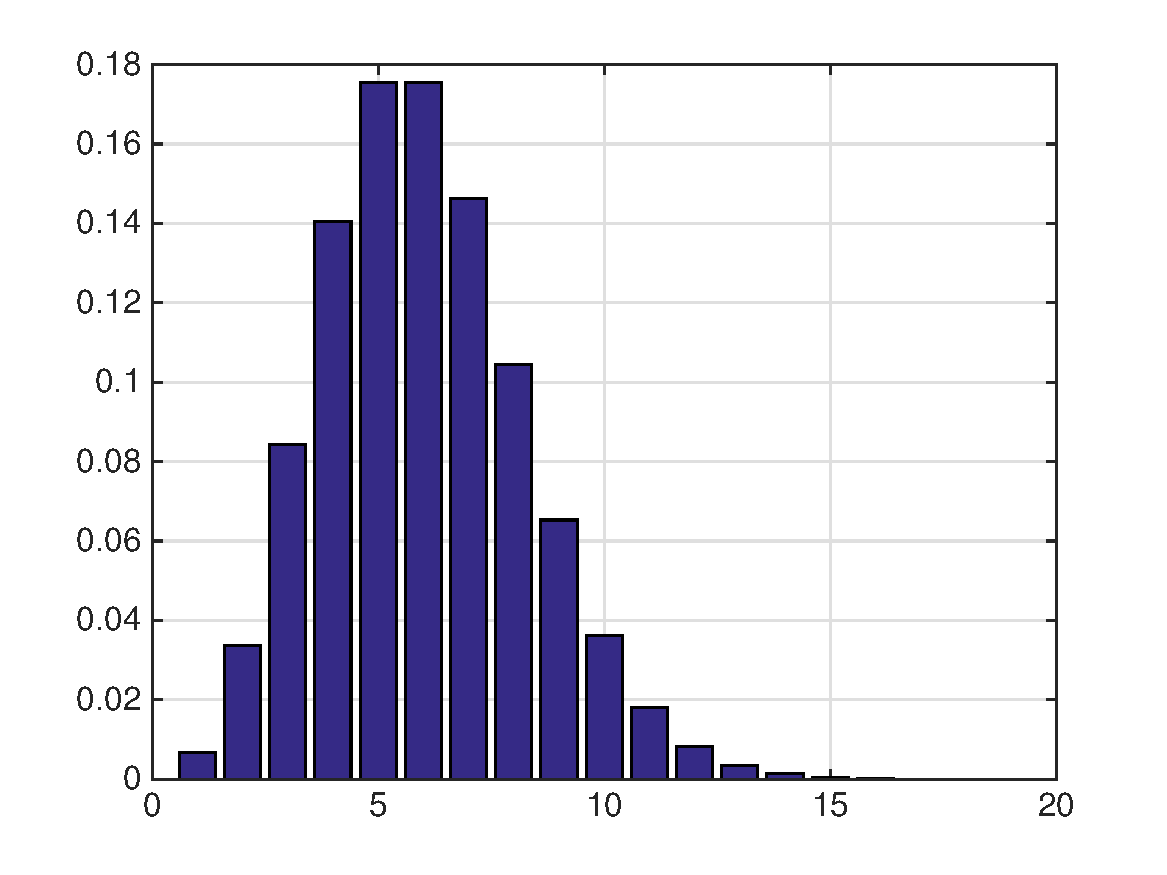
\includegraphics[scale=0.35]{poisson}
\caption{The Poisson distribution with $\lambda = 5$.}
\label{fig:poisson}
\end{figure}



\subsubsection*{Poisson and Coin Flips}

To see a concrete example of how Poisson distribution arises, suppose we want to model the number of cell phone
users initiating calls in
a network during a time period, of duration (say) 1 minute. There are many customers in the network,
and all of them can potentially make a call during this time period. However, only a very small fraction of
them actually will. Under this scenario, it seems reasonable to make two assumptions:
\begin{itemize}
\item The probability of having more than 1 customer initiating a call in any small time interval is negligible.
\item The initiation of calls in disjoint time intervals are independent events.
\end{itemize}
Then if we divide the one-minute time period into $n$ disjoint intervals, then the number of calls $X$ in that
time period can be modeled as a binomial random variable with parameter $n$ and probability of success $p$, i.e., $p$ is the
probability of having a call initiated in a time interval of length $1/n$. But what should $p$ be in terms of
the relevant parameters of the problem? If calls are initiated at an average rate of $\lambda$ calls per minute, then
$\Ex{X} = \lambda$ and so $np = \lambda$, i.e., $p = \lambda/n$ . So $X \sim Bin(n,\frac{\lambda}{n})$. As we shall see
below, as we let $n$ tend to infinity, this distribution tends to the Poisson distribution with parameter $\lambda$.
We can also see why the Poisson distribution is a model for ``rare events.'' We are thinking of it as a sequence of 
a large number, $n$, of coin flips, where we expect only a finite number $\lambda$ of Heads. 

Now we will prove that the Poisson distribution $Poiss(\lambda)$ is the limit of the binomial distribution $Bin(n, \frac{\lambda}{n})$, as $n$ tends to infinity.

\begin{theorem}
Let $X \sim Bin(n, \frac{\lambda}{n})$ where $\lambda > 0$ is a fixed constant. Then for every $i = 0,1,2,\dots$,
$$\Pr[X = i] \longrightarrow \frac{\lambda^i}{i!} \e^{-\lambda} ~~~ \text{ as } ~ n \to \infty.$$
That is, the probability distribution of $X$ converges to the Poisson distribution with parameter $\lambda$.
\end{theorem}
\begin{proof}
Fix $i \in \{0,1,2,\dots\}$, and assume $n \ge i$ (because we will let $n \to \infty$). Then, because $X$ has binomial distribution with parameter $n$ and $p = \frac{\lambda}{n}$,
$$\Pr[X = i] = {n \choose i} p^i (1-p)^{n-i}
= \frac{n!}{i! (n-i)!} \left(\frac{\lambda}{n}\right)^i \left(1-\frac{\lambda}{n}\right)^{n-i}.$$
Let us collect the factors into
\begin{equation}\label{eq:binpoiss}
\Pr[X = i]
= \frac{\lambda^i}{i!} \left( \frac{n!}{(n-i)!} \cdot \frac{1}{n^i} \right) \cdot \left(1-\frac{\lambda}{n}\right)^n \cdot \left(1-\frac{\lambda}{n}\right)^{-i}.
\end{equation}
The first parenthesis above becomes, as $n \to \infty$,
$$\frac{n!}{(n-i)!} \cdot \frac{1}{n^i} = \frac{n \cdot (n-1) \cdots (n-i+1) \cdot (n-i)!}{(n-i)!} \cdot \frac{1}{n^i}
= \frac{n}{n} \cdot \frac{(n-1)}{n} \cdots \frac{(n-i+1)}{n}
\to 1.$$
From calculus, the second parenthesis in~\eqref{eq:binpoiss} becomes, as $n \to \infty$,
$$\left(1-\frac{\lambda}{n}\right)^n \to \e^{-\lambda}.$$
And since $i$ is fixed, the third parenthesis in~\eqref{eq:binpoiss} becomes, as $n \to \infty$,
$$\left(1-\frac{\lambda}{n}\right)^{-i} \to (1-0)^{-i} = 1.$$
Substituting these results back to~\eqref{eq:binpoiss} gives us
$$\Pr[X = i]
\to \frac{\lambda^i}{i!} \cdot 1 \cdot \e^{-\lambda} \cdot 1 = \frac{\lambda^i}{i!} \e^{-\lambda},$$
as desired.
\end{proof}


\end{document}
